\section{Computational Biology} 
 
\textit{Computational Biology} is defined as the development and application of data-analytical and theoretical methods, mathematical modeling and computational simulation techniques to the study of biological, behavioral, and social systems\cite{1}.

The field is now thirty years old and it's covered by many conferences and journals publishing papers. It features graph theory, network flows, combinatorics, integer and linear programming problems, statistical approaches, probabilistic methods, hidden Markov models, neural networks as its tools.

Some of the most important challenges are\cite{Searls19983}:
\begin{itemize}
\item Protein structure prediction.
\item Homology searches.
\item Multiple alignment and phylogeny construction.
\item Genomic sequence analysis and gene-finding.
\end{itemize}

In particular, \textit{Computational Molecular Biology} (bioinformatics) focuses on studying existing and emerging approaches, techniques and algorithms for string computation (sequences) providing a significant intersection between computer science and molecular biology \cite{Gusfield:1997:AST:262228}.

For these reasons, the field is inherently multidisciplinary: it's appealing to the Mathematical Programming and Operations Research community. 
Today, computational biology papers are written by computer scientists, biologists, statisticians, physicists and mathematicians, pure and applied.
\clearpage
\paragraph{}
Concretely, the application areas are \cite{a1020100}:
\begin{itemize}
	\item \textsc{Evolution.} Comparison of whole genomes to highlight evolutionary macro events (inversions, transpositions, translocations). Computation of evolutionary distances between genomes. Computation of common evolutionary subtrees or of evolutionary supertrees.
		\begin{figure}[h]
  \centering
    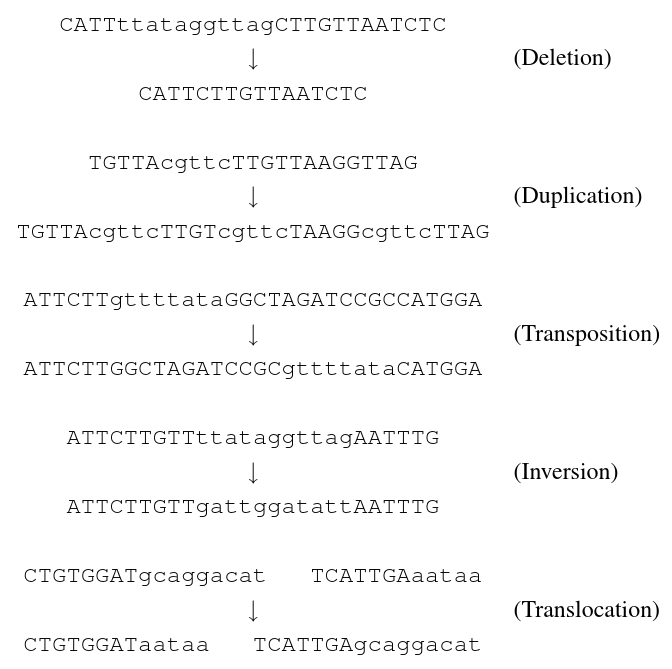
\includegraphics[width=250pt]{evolutionary_events}
  \caption{Five types of evolutionary events}
\end{figure}
	\item \textsc{Sequence analysis.} Comparison of genomic sequences within individuals of a same species, or intra-species, in order to highlight their differences and similarities. Reconstruction of long sequences by assembly of shorter sequence fragments. Error correction for sequencing machines.
	\item \textsc{Hybridization and microarrays.} Use of hybridization for sequencing. Use of microarrays for tissue identification, clustering and feature selection discriminating healthy from diseased samples. Design of optimal primers for PCR experiments. Physical mapping (ordering) of probes by hybridization experiments.
	\item \textsc{Protein structures.} Protein fold prediction from aminoacid sequence (ab-initio), or from sequence + other known structures (threading of sequences to structures). Alignment of RNA sequences depending on their structure. Protein fold comparison and alignment of protein structures. Study of protein docking and synthesis of molecules of given 3D structure.
	\item \textsc{Haplotyping.} (DNA mutations) Reconstruction and/or correction of haplotypes from partial haplotype fragments or from genotype data. Analysis of resulting haplotypes and correlation with genetic diseases \cite{Bonizzoni2003}.

\end{itemize}



Note that the term \textit{bioinformatics} is used also as an umbrella term for the (wider) body of biological studies using computer programming as part of their methodology, as well as a reference to specific analysis "pipelines" that are repeatedly used, particularly in the field of genomics.